\documentclass{article}

\usepackage[french]{babel}
\usepackage[T1]{fontenc}
\usepackage{moreverb}       % verbatim with tab

\usepackage{wrapfig}
\usepackage{graphicx}
\usepackage{geometry}
\geometry{hmargin=2.5cm}
\usepackage{amsmath}
\usepackage{siunitx}

\usepackage{graphicx}
\usepackage{subcaption}
\usepackage{float}
\usepackage{hyperref}
\usepackage{setspace}
\usepackage{xcolor}
\usepackage{pdfpages}
\usepackage{enumitem}
\usepackage{lscape}

\usepackage{fancyhdr}       % en-têtes
\usepackage{lastpage}       % numéro de dernière page

\title{Systèmes logiques programmés\bigbreak \bigbreak
    \large Dossier récapitulatif\bigbreak
    \normalsize Programmation d'un générateur de signaux en assembleur sur PIC16F887\bigbreak}
\date{2020 -- 2021}
\author{Laura Binacchi}

\pagestyle{fancy}
\renewcommand\headrulewidth{1pt}
\fancyhead[L]{Laura Binacchi}
\fancyhead[C]{Systèmes logiques programmés}
\fancyhead[R]{\today}


\begin{document}
    \pagenumbering{gobble}
    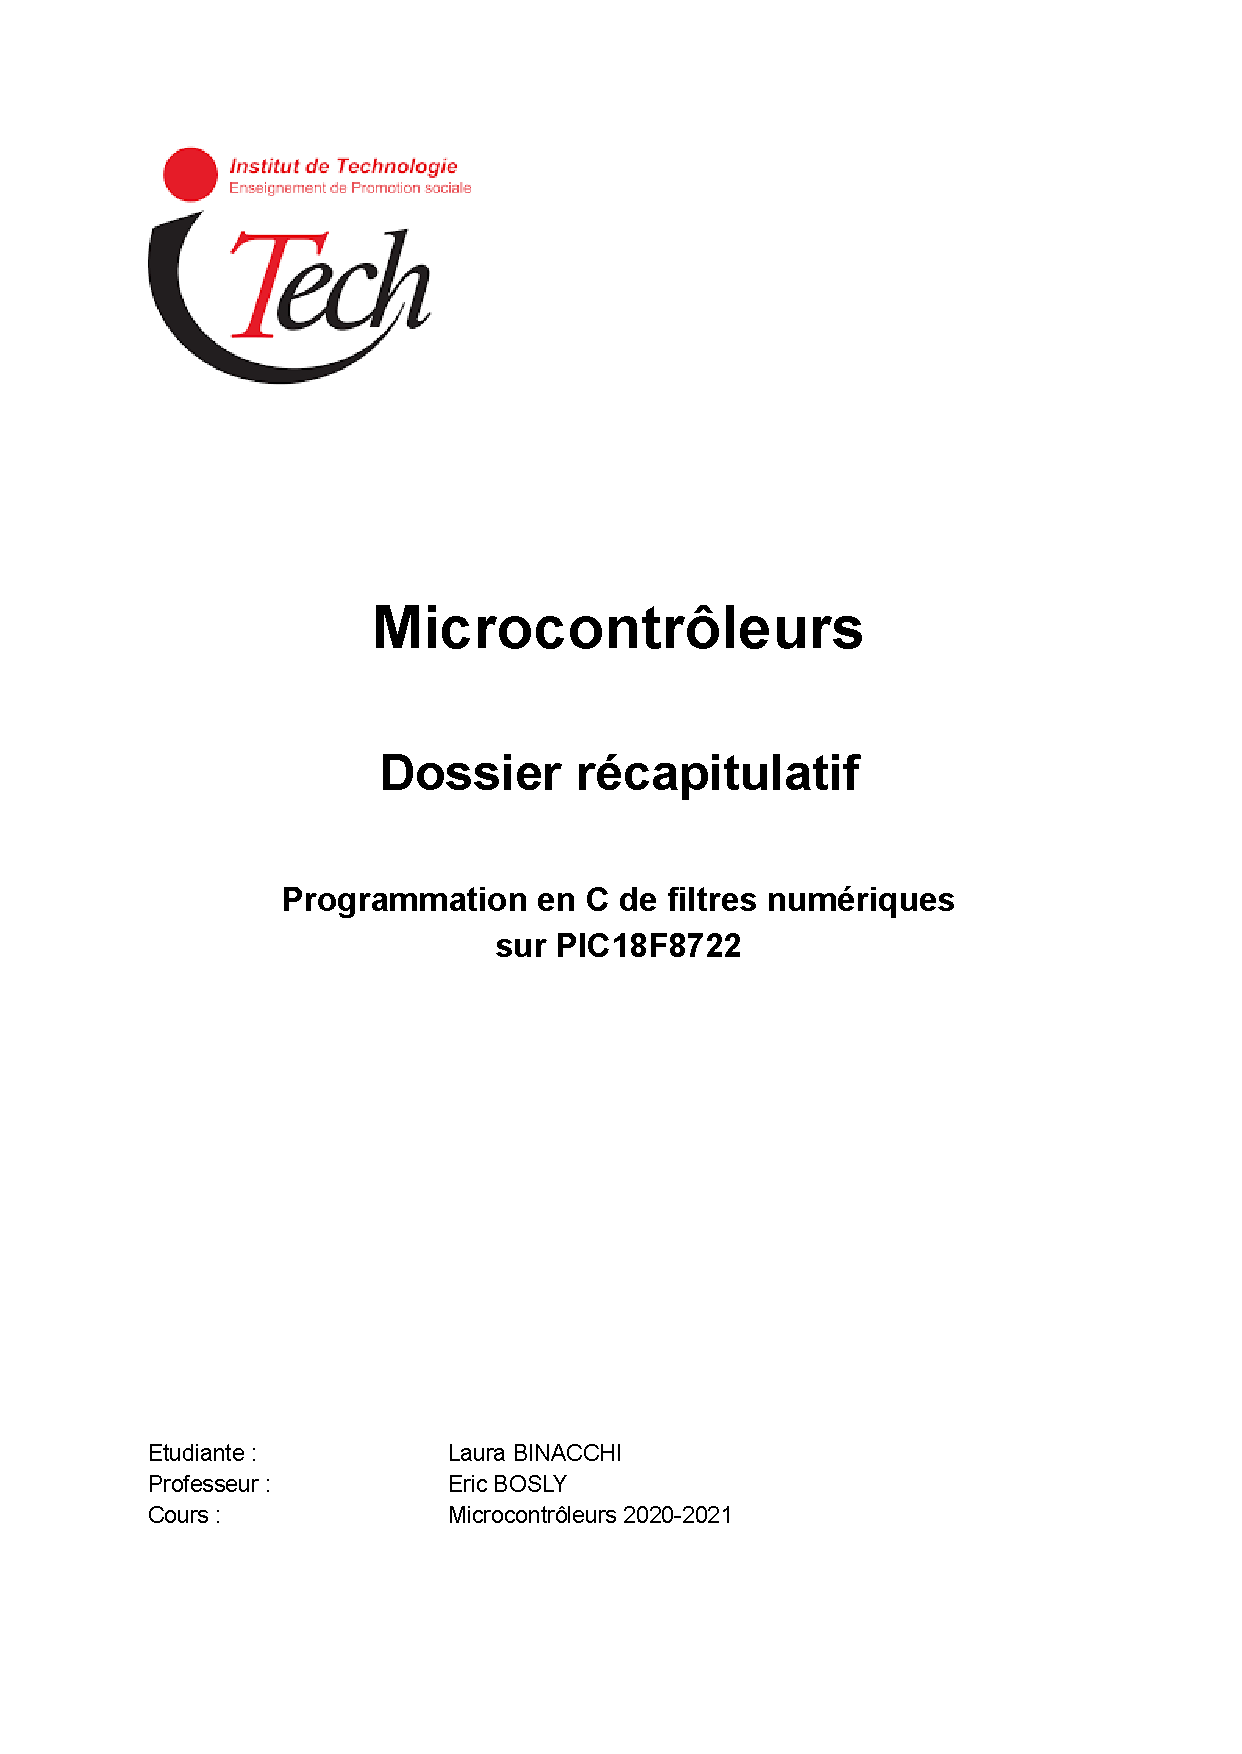
\includepdf[pages={1}]{pdg}
    \newpage
    \tableofcontents
    \newpage
    \pagenumbering{arabic}

    \section{Cahier des charges}

    \subsection{Travail demandé}
    \paragraph{}
    Ecrire un programme en langage C sous MPLABX XC8 pour filtrer un signal sonore mono envoyé à partir d’un fichier .wav sur l’entrée analogique d’un PIC. Ce programme devra tourner sur un PIC18F8722 en simulation Proteus. Ce PIC pilotera un convertisseur NA de sortie permettant d’écouter le résultat des filtres. On respectera les règles de bonne syntaxe vues au cours, notamment en termes de commentaires.

    \paragraph{}
    Un fichier Proteus d’exemple et des fichiers son ont été fournis. L’interface utilisateur du programme est laissée à l’appréciation du développeur, je propose ci-dessous un menu circulaire utilisant le LCD et des boutons poussoirs. Ne perdez cependant pas trop de temps dans ce domaine, ce n’est pas le principal. Le plus important dans ce dossier, sera la mise au point des quatre filtres demandés, programmation et tests.

    \subsection{Cahier des charges de l’application}
    \paragraph{}
    Un signal sonore en mono, généré par une application de type Audacity avec une fréquence d’échantillonnage de 8 ou 16 kHz, est injecté sur une entrée analogique du PIC. Le signal est numérisé sur 8 bits par le module CAN du PIC et filtré en temps réel selon le mode de fonctionnement courant. Le signal filtré est recomposé par un CNA MCP4922 ou DAC0808 au choix, à piloter. Le résultat est audible dans un graphe audio, exportable.

    \paragraph{}
    Connecter un afficheur LCD 4 lignes de 20 caractères, le programme aura plusieurs modes de fonctionnement, résumés dans le tableau ci-dessous.

    \paragraph{}
    La fréquence d’échantillonnage $F_e$ du signal sera configurable à 8kHz ou 16kHz. La fréquence d’échantillonnage conditionne évidement les fréquences de coupure des filtres.

    \paragraph{}
    Le mode « Configuration » et les menus sont laissés à l’appréciation du concepteur. Attention aux conflits potentiels entre le LCD et le convertisseur CNA, si ils utilisent tous les deux une connexion SPI.

    \subsection{Description des 4 filtres demandés}

    \begin{tabular}{l l l}
        Variables           & Y : tampon sortie & X : tampon entrée \\
                            & N : dimension du tampon & \\
                            & A, B : coefficients & \\
                            & & \\
        Moyenne glissante   & $Y_j = \sum\limits_{i=0}^{N-1} \frac{X_{j-i}}{N}$ & pour N = 2 à 8 \\
                            & & \\
        Filtre récursif     & $Y_j = \sum\limits_{i=0}^{N-1} A_i X_{j-i} - \sum\limits_{i=1}^{N-1} B_i X_{j-i}$ & voir fichier tableur joint \\
                            & & \\
        Echo                &  $Y_j = A X_j + B X_{j-del}$ & avec $A + B = 1$ \\
    \end{tabular}

    \paragraph{}
    Le menu décrit ci-dessous est exemplatif, pour éviter de perdre trop de temps avec Proteus, vous pouvez limiter la complexité de l’interface homme-machine.


    \begin{figure}[H]
        \centering
        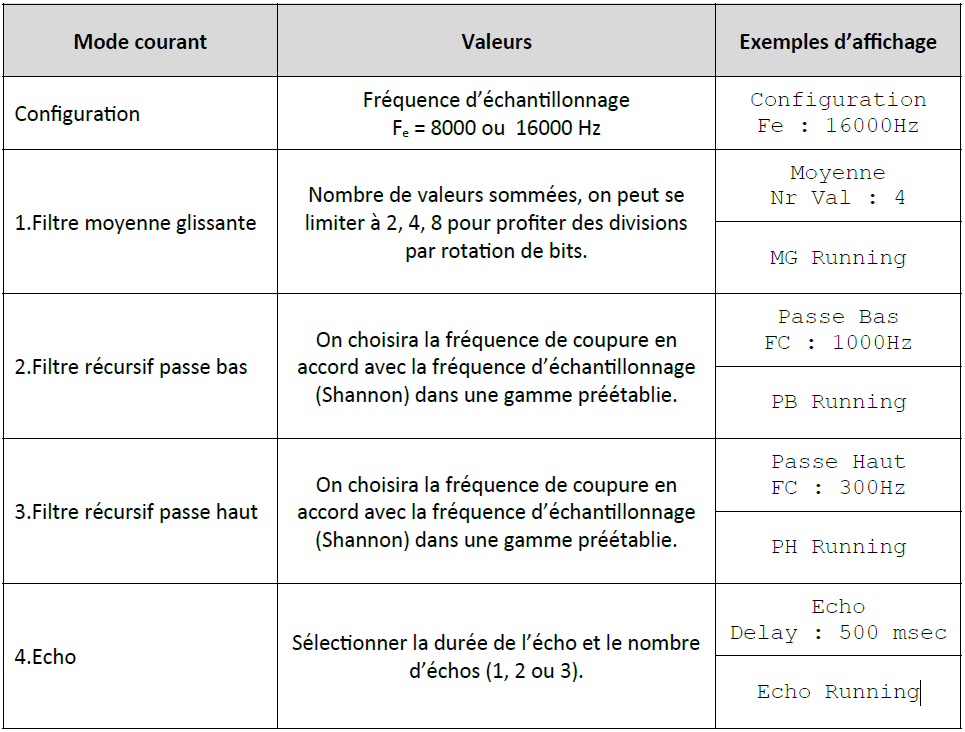
\includegraphics[width=.7\textwidth]{./images/menus.png}
    \end{figure}


    % Moyennes glissantes : implémenter des pas en puissance de 2 permet d'implementer une frequence d'echantillonnage plus elevee, i.e. 16k au lieu de 8 car la rotation de bits est plus rapide que

    % Remarques sur le projet Proteus
    % pas de filtre anti aliasing car l'audio d'entrée est déjà échantillonné à la bonne fréquence (sinon on pourrait rajouter un filtre de laplace aussi en entrée). Mais ici, la simulation est déjà assez lente...

    % Attention pour les analyses de Fourier : bien setter la fréquence max à la fréquence utile du signal (-> Fe/2), changer aussi la fréquence de coupure du filtre


    % Cahier des charges : c'est mieux de
    % - mettre au point un menu circulaire
    % - connecter le MCP que le DAC (attention aux conflits avec de LCD)

    % Dans le travail : mettre en avant les réglages du filtre et les effets sur le signal. Attention, plus le filtre est filtrant, plus le signal de sortie est déphasé -> le signal est plus lisse (beau) mais déphasé
    % Mettre en avant l'utilisation du tick et de l'oscilloscope.


    \newpage
    \section{Organigramme de haut niveau}
    \begin{figure}[H]
        \centering
        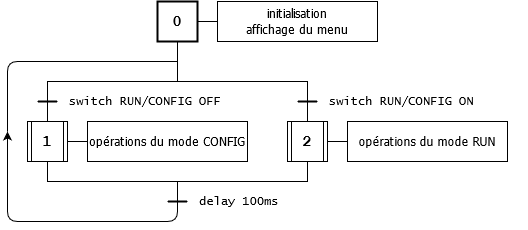
\includegraphics[width=.5\textwidth]{./images/orga_global.png}
        \caption{Organigramme : boucle principale}
    \end{figure}

    \paragraph{}
    Le programme démarre par l'initialisation du PIC \textbf{[0]}. La configuration du PIC et des périphériques (écran LDC et DAC) est détaillée dans la section~\ref{section:configuration}. Les paramètres de traitement du signal et les variables de gestion du menu sont initialisés avec des valeurs par défaut définies pour la plupart (quand cela est possible) par des variables du préprocesseur. Puis le menu est affiché sur l'écran LCD :
    \begin{itemize}
        \item le type de filtre est affiché sur la première ligne;
        \item la fréquence d'échantillonnage est affichée sur la deuxième ligne;
        \item les paramètres du filtre sont affichés sur la troisième et, uniquement dans le cas du filtre echo, sur la quatrième ligne.
    \end{itemize}

    \begin{figure}[H]
        \centering
        \begin{subfigure}[b]{0.34\textwidth}
            \centering
            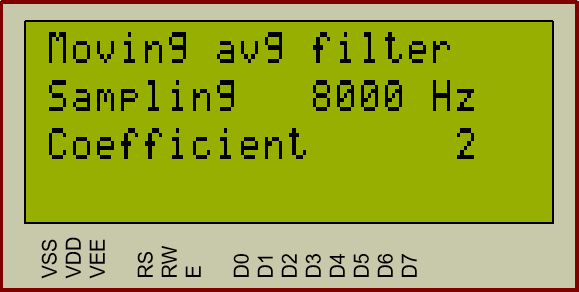
\includegraphics[width=.9\textwidth]{./images/vue_mov_avg.png}
            \caption{Filtre par moyenne glissante}
        \end{subfigure}
        \begin{subfigure}[b]{0.34\textwidth}
            \centering
            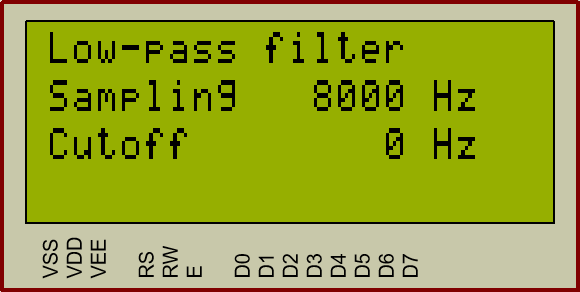
\includegraphics[width=.9\textwidth]{./images/vue_low_pass.png}
            \caption{Filtre passe-bas}
        \end{subfigure}
        \begin{subfigure}[b]{0.34\textwidth}
            \centering
            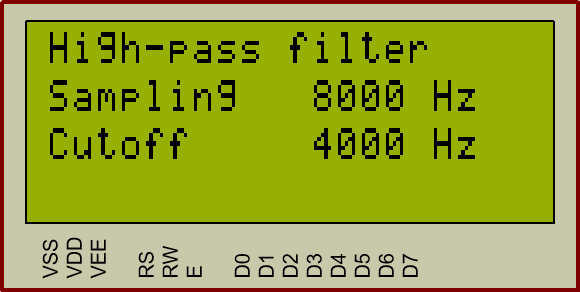
\includegraphics[width=.9\textwidth]{./images/vue_high_pass.png}
            \caption{Filtre passe-haut}
        \end{subfigure}
        \begin{subfigure}[b]{0.34\textwidth}
            \centering
            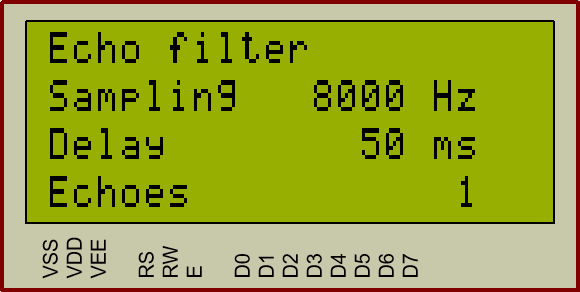
\includegraphics[width=.9\textwidth]{./images/vue_echo.png}
            \caption{Filtre echo}
        \end{subfigure}
        \caption{Vues des différents menus}
   \end{figure}

    \paragraph{}
    En fonction de l'état du switch \texttt{RUN}/$\overline{\texttt{CONFIG}}$, le programme fonctionne soit en mode de configuration \textbf{[1]}, soit en mode de traitement du signal \textbf{[2]}. L'état du switch est scanné en boucle après l'exécution des instructions du mode de fonctionnement sélectionné et une temporisation de \SI{100}{\milli\second}.

    \subsection{Mode de configuration}
    \begin{figure}[H]
        \centering
        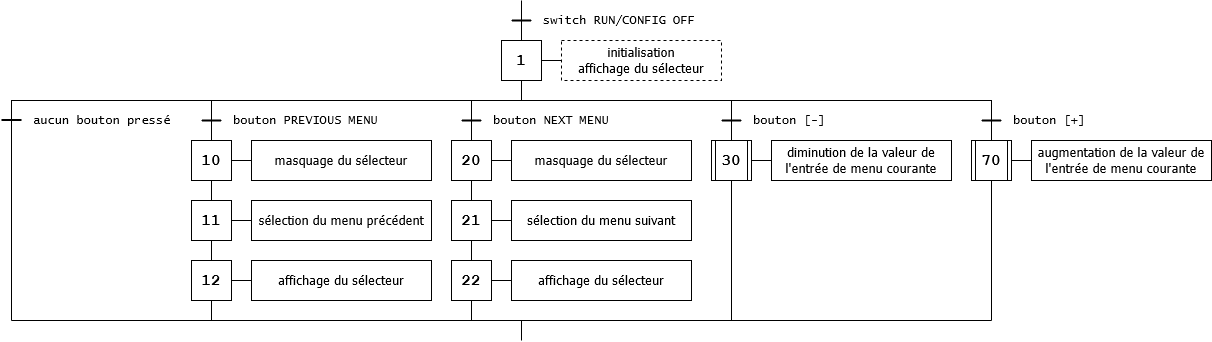
\includegraphics[width=\textwidth]{./images/orga_config.png}
        \caption{Organigramme : mode de configuration}
    \end{figure}

    \paragraph{}
    A son initialisation \textbf{[1]}, le mode de configuration désactive les interruptions de haute priorité, i.e. le traitement du signal, l'entrée de menu active est initialisée au type de filtre et le sélecteur de menu \texttt{<} est affiché sur la ligne correspondante. Grâce à une variable conservant l'état précédant du switch \texttt{RUN}/$\overline{\texttt{CONFIG}}$, le mode de configuration n'est initialisé que lors du passage du mode RUN vers le mode CONFIG.

    \paragraph{}
    Les différents boutons de paramétrage du filtre sont scannés un à un. Si aucun bouton n'est pressé, le programme continue de scanner les entrées tant que le mode de configuration est actif. Si plusieurs boutons sont pressés en même temps, seul le premier est pris en compte selon l'ordre dans lequel ils sont scannés.

    \paragraph{}
    Les boutons \texttt{PREVIOUS} et \texttt{NEXT} permettent de naviguer dans le menu. Lorsque le bouton \texttt{PREVIOUS} est pressé puis relâché, le sélecteur de menu est effacé \textbf{[10]}. L'entrée de menu précédente est sélectionnée \textbf{[11]} en mettant à jour la variable du programme qui garde en mémoire l'entrée de menu courante. Puis le sélecteur est affiché sur la nouvelle entrée active \textbf{[12]}. Si la première entrée du menu est active lorsque le bouton \texttt{PREVIOUS} est pressé, c'est la dernière entrée du menu qui devient active.

    \begin{figure}[H]
        \centering
        \begin{subfigure}[b]{.34\textwidth}
            \centering
            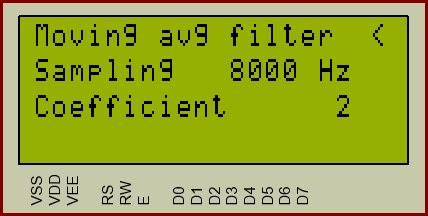
\includegraphics[width=.9\textwidth]{./images/previous_a.png}
        \end{subfigure}
        \begin{subfigure}[b]{.34\textwidth}
            \centering
            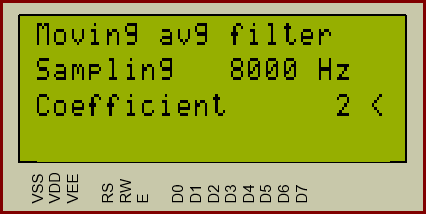
\includegraphics[width=.9\textwidth]{./images/previous_b.png}
        \end{subfigure}
        \caption{Passage du sélecteur de la première à la dernière entrée lorsque le bouton \texttt{PREVIOUS} est pressé}
    \end{figure}

    \paragraph{}
    De la même manière, lorsque le bouton \texttt{NEXT} est pressé puis relâché, le sélecteur de menu est effacé \textbf{[20]}, l'entrée de menu suivante est sélectionnée \textbf{[21]} puis le sélecteur est affiché sur la nouvelle entrée de menu active \textbf{[22]}.

    \paragraph{}
    Les boutons \texttt{[-]} et \texttt{[+]} permettent de modifier le type de filtre et ses paramètres en diminuant \textbf{[30]} ou augmentant \textbf{[70]} la valeur de l'entrée de menu active.

    \begin{figure}[H]
        \centering
        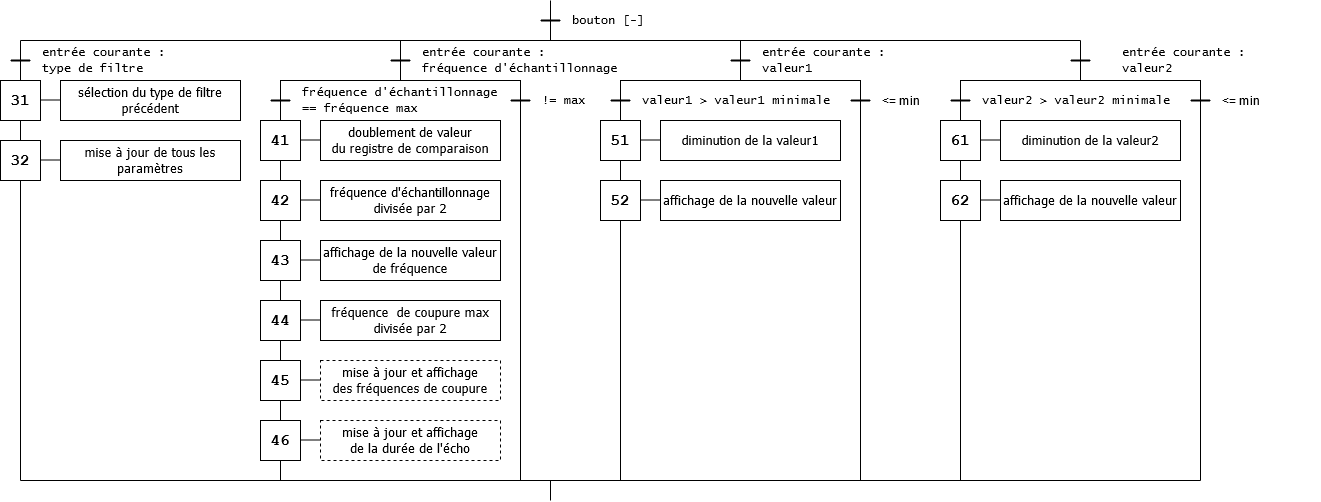
\includegraphics[width=\textwidth]{./images/orga_decrease.png}
        \caption{Organigramme : diminution de la valeur de l'entrée de menu active}
    \end{figure}

    \paragraph{}
    La modification du type de filtre \textbf{[31]} se fait, comme la navigation, de manière circulaire : il tourne en boucle en appuyant sur le bouton \texttt{[+]} ou sur le bouton \texttt{[-]}, dans un sens de défilement ou dans l'autre. Lorsque le type de filtre est modifié, c'est tout l'affichage qui est mis à jour \textbf{[32]} car les paramètres configurables dépendent du type de filtre actif.

    \paragraph{}
    La fréquence d'échantillonnage n'a que deux valeurs possibles : \SI{8}{\kilo\hertz} ou \SI{16}{\kilo\hertz}. Elle n'est donc diminuée que si elle est au maximum (de la même manière, elle ne sera augmentée que si elle est au minimum). La valeur de comparaison de l'interruption est doublée \textbf{[41]} et la valeur de la fréquence d'échantillonnage est divisée par deux \textbf{[42]} puis mise à jour sur le LCD \textbf{[43]}. La fréquence d'échantillonnage détermine la fréquence de coupure maximale qui peut être utilisée par les filtres : ce maximum est fixé à la moitié de la fréquence d'échantillonnage \textbf{[44]} (théorème de Shannon). Si les fréquences de coupure des filtres passe-bas et passe-haut dépassent cette valeur maximale, elles prennent cette nouvelle valeur et, si filtre actif est un filtre passe-bas ou passe-haut, le LCD est mis à jour \textbf{[45]}.

    \paragraph{}
    La diminution de la première valeur met à jour \textbf{[51]}, en fonction du filtre actif, soit : le coefficient du filtre par moyenne glissante; la fréquence de coupure du filtre passe-bas; la fréquence de coupure du filtre passe-haut; le délai du filtre echo.

    \paragraph{}
    La deuxième valeur \textbf{[61]} ne concerne que le filtre echo et met à jour le nombre d'echos.

    \paragraph{}
    Ces valeurs ne peuvent être diminuées que si elles sont strictement supérieures aux valeurs minimales définies par des variables du préprocesseur. Elles sont diminuées d'un pas également défini par des variables du préprocesseur. Le même mécanisme est implémenté pour l'augmentation des valeurs.

    \subsection{Mode de traitement du signal}
    \begin{figure}[H]
        \centering
        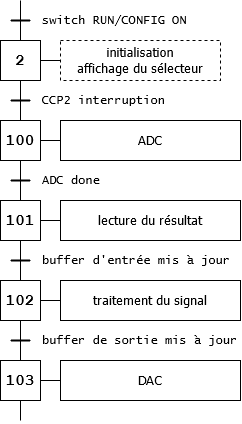
\includegraphics[width=.2\textwidth]{./images/orga_run.png}
        \caption{Organigramme : mode de traitement du signal}
    \end{figure}

    \paragraph{}
    Comme le mode de configuration, le mode de traitement du signal n'est initialisé que lors du passage du mode \texttt{CONFIG} au mode \texttt{RUN} \textbf{[2]} : le sélecteur de menus \texttt{<} est masqué et le signal est initialisé en fonction du type de filtre actif et de ses paramètres.

    \paragraph{}
    Une interruption survient toutes les \SI{1250}{\micro\second} (fréquence d'échantillonnage à \SI{8}{\kilo\hertz}) ou toutes les \SI{625}{\micro\second} (fréquence d'échantillonnage à \SI{16}{\kilo\hertz}). Elle déclenche la conversion analogique-numérique (ADC) \textbf{[100]}. Quand elle est terminée, son résultat est lu dans le tampon d'entrée \textbf{[101]}. Le signal est alors traité selon le type de filtre et ses paramètres \textbf{[102]} et la résultat du traitement est placé dans le tampon de sortie pour pouvoir être transmis au convertisseur numérique analogique (DAC) \textbf{[103]}.








    % Ici il y aurait eu un intérêt à faire comme dans le projet de SLP : connecter les boutons à un I/O expander SPI qui déclencherait une interruption de priorité plus faible que l'interruption qui génère le signal. Dans ce cas, il aurait également fallu veiller à mettre des verrous sur les opérations de communication SPI pour qu'elles puissent se dérouler correctement sans interruption. Cette remarque s'applique particulièrement dans le cas ou un MCP4922 est utilisé plutôt qu'un DAC0808 puisque la communication entre le PIC et le DAC dans l'interruption principale se fait via un bus SPI.


    \newpage
    \section{Fréquences utilisées}
    % La description et la justification des fréquences utilisées
    % Fréquence d'échantillonnage, fréquence utile du signal et fréquence de coupure du filtre de Laplace (entre max Fs/2 et min la fréquence du signal: à la moitié de la fréquence d'échantillonnage, c'est ok pour toutes les fréquences de signaux mais pour mieux lisser, on peut jouer avec la fréquence de coupure du filtre pour la rapprocher de la fréquence du signal, d'autant plus qu'ici on a un filtre de Laplace, d'ordre 1, i.e. un simple RC qui a donc une faible sélectivité, i.e. la coupure n'est pas nette)
    % Remarque : le filtre de Laplace déphase le signal de sortie d'autant plus qu'il est plus filtrant.

    \section{Configuration du PIC}
    \label{section:configuration}
    % La description de la configuration du PIC utilisée
    % DAC0808 banché directement sur le port D plutôt que via un bus de communication (SPI ou I2C) -> plus rapide -> fréquence d'échantillonnage + élevée (50 kHz au lieu de 20kHz via SPI)

    % \paragraph{MCP4922}
    % Dual 12-Bit Voltage Output DAC -> intéressant si on veut passer le programme en stereo même si permet une fréquence de signal plus petit qu'un DAC connecté directement au PIC (SPI Interface with 20 MHz Clock Support -> suffisant pour le 16k ici)

    % Utilisation d'un seul channel en 8bits (mode x2) : he  user
    % can  configure  the  full-scale  range  of  the  device  to  be
    % VREF or 2 * VREF by setting the Gain Selection Option
    % bit (gain of 1 of 2)

    % améliorations :
    % - utilisation du mode shutdown quand le programme est en mode configuration
    % SHDN is the hardware shutdown input pin. When this
    % pin  is  low,  both  DAC  channels  are  shut  down.  DAC
    % output is not available during the shutdown.
    % - setter voutb à sutdown (cf p.24)

    % VDD entre 2,7 et 5,5V
    %It is recommended to use an appropriate bypass
    %capacitor  of  about  0.1 μF  (ceramic)  to  ground.  An
    %additional 10 μF capacitor (tantalum) in parallel is also
    %recommended to further attenuate high frequency
    %noise present in application boards.

    % CS active à l'état bas -> configuration tris en output et set à 1. Idem pour LDAC (load pin qui transfère le registre vers les pin d'output)

    % SCK -> sck

    % sdi -> sdo


    % lA TENSION DE SORTIE $V_{OUT} = \frac{V_{REF} \times D_n}{2^n} G$
    % ici le gain est de 2 (mode x2 GA à 0), VRef est à VDD -> 5V, Dn = input et n = résolution (ici 12 bits)

    % -> $V_{OUT} = \frac{5 \times D_n}{2048}$ -> Dn varie entre 0 et 255 (car utilisé max à 8 bits ici) -> vout varie entre 0 et 0,62V (vérifié à l'oscillo -> ok)


    \paragraph{Filtre numérique}
    %https://fr.wikipedia.org/wiki/Filtre_num%C3%A9rique
    %http://mustig.free.fr/fr/doc/exemples_commentes/doc/fil_rec.htm
    Forme générale (normalisée) des filtres numériques d'ordre M :
    $$ y[N] = \sum\limits_{k=0}^{N} b_k \times x_{n-k} - \sum\limits_{k=1}^{M} a_k y_{n-k} $$
    $$ Y_j = \sum\limits_{i=0}^{N-1} A_i X_{j-i} - \sum\limits_{i=1}^{N-1} B_i X_{j-i} $$

    \paragraph{Filtre moyenne glissante}
    Filtre à réponse impulsionnelle finie (FIR: finite impulse response) dont le coefficient $a = \frac{1}{N}$ et $b = 0$


    \section{Tests}
    % La description des tests à effectuer pour valider le programme

    \section{Difficultés rencontrées}
    % Le calcul des mises à échelle pour s'assurer qu'il n'y a pas de dépassement de valeurs.


    % \section{Configuration}
    % \paragraph{Conversion analogique-digitale (A/D conversion)}
    % ADCON0 permet de :
    % - activer la conversion (bit ADON)
    % - vérifier quand la conversion est faite (bit GO/DONE)
    % - sélectionner l'entrée analogique liée à l'ADC

    % ADCON1 :
    % permet de
    % - configurer les entrées en analogique ou digital (TOR)
    % Par défaut, tout est analogique. Ici on sera en 1101 (AN0 AN1), éventuellement 1011 (de AN0-3, AN2-3 étant des PIN de tension de ref) -> attention aux PIN en TOR dont on a besoin
    % - configurer les tensions de référence du module ADC et d'où elles viennent
    % Pour le programme, on travaille en mode 0 (mode par défaut), i.e. tensions de référence sur VDD et VSS (entre 0 et 5V)

    % ADCON2
    % gère le fonctionnement technique du module ADC, dont
    % - sa justification à droite ou à gauche (bit ADFM)
    % - la configuration du temps d'acquisition (ACQT<2:0>)
    % - la configuration de la fréquence de conversion, dérivée par rapport à la fréquence de l'oscillateur (ADCS<2:0>)

    % ADRESH et ADRESL
    % contiennent le résultat de la conversion


    % 1 Entrées analogiques ou digitales ? -< configuration de ADCON1

    % 2 Tensions de référence ? -> 00

    % 3 Temps de conversion ? il faut 12 temps TAD avant de finir la conversion et d'avoir le déclenchement du GO/DONE
    % valeur min de TAD = 0,7us
    % valeur de TAD fixé par le quartz et les bits ADCS<2:0> de l'ADCON2

    % à 10MHz HSPLL, 1 tosc = 0,1us
    % puisqu'il faut min 0,7us => il faut choisir le 8tosc (001)

    % => le temps de conversion va durer 12*8TOSC = 0,96us
    % => on peut tenir une fréquence théorique max de 100kHz
    % (limite théorique mais en pratique on doit aller moins vite pour garder de la puissance processeur pour autre chose)

    % 4 Temps d'acquisition ? ACQT<2:0>
    % typiquement, dans un système qui ne fait pas que de la conversion, on le laisse à 0 parce que le temps de conversion est là en ayant fait autre chose avant.

    % 5 Justification de résultat ? ADFM
    % 8 bits -> à gauche et on utilise que adresh
    % 10 bits -> à droite et on utilise adresh et l

    % 6 Choix du canal de conversion ? ADCON0
    % Ici avec Proteus on n'est pas limité par un hardware déjà soudé

    % 7 Alimentation du CAN ?
    % Dernière étape : activer l'ADC avec le bit ADON

    % Utilisation : on met 1 dans le GO/DONE et on attend que ça saute pour avoir le résultat

    % Code d'exemple
    % fréquence d'échantillonnage de 20kHz



    % Filtre echo :
    % Paramètres :

    % - poids de l'echo (weight)
    % -> 22/02 (fin)

    % 1/03 interruptions prioritisées



    % \section{Fonctionnement du programme}



    % \section{Tests}



    % \section{Problèmes rencontrés}



\end{document}